\section{Problem Formulation}
It is difficult to operate high end CAD software for a simple layman as he does not have  much knowledge of the computer system because they are not connected to the internet in any ways. Giving training to these peoples is not easy as there is not so much manpower available to provide training and it will be expensive also. By not using the computer softwares instead of traditional drawing methods, Resources are being wasted 
on manually making the drawings at various levels.
Also it is very difficult to make the drawing design using the traditional methods these days because of the evolving computer CAD softwares. \\

\noindent The pencil and paper work can be reduced to a great extent by doing the drawing work using Automated Building Drawings system making it environment friendly. Thus, making it automated process. Lot of time was wasted standing in the previous processes of making a drawing, but now with this system we have a facility to do it in an easy way. The previous process was quite difficult and time consuming. The laymen which were not quite familiar with the popular CAD softwars always found it difficult to make their design using these softwares which leads them to use the paper and pencil method for drawings. Now with the cration of this system they can easily make the desired designs and also can increase their productivity by reducing the time required.


\section{Feasibility Study}
\noindent Feasibility analysis involved a thorough assessment of the operational and technical aspects of the proposal.
Feasibility study tested the system proposal and identified whether the user needs may be satisfied using
the current software and hardware technologies, whether the system will be cost effective from a business
point of view and whether it can be developed with the most up to date technologies.
\subsection{Operational Feasibility}
\noindent Operational feasibility is a measure of how well a project solves the problems, and takes advantage of
the opportunities identified during scope definition and how it satisfies the requirements identified in
the requirements analysis phase of system development. All the operations performed in the software
are very quick and satisfy all the requirements.
\subsection{Technical Feasibility}
\noindent Technological feasibility is carried out to determine whether the project has the capability, in terms
of software, hardware, personnel to handle and fulfill the user requirements. The assessment is based
on an outline design of system requirements in terms of Input, Processes, Output and Procedures.
Automated Building Drawings is technically feasible as it is built up using various open source technologies and it can run on any platform.
\subsection{Economic Feasibility}
\noindent Economic analysis is the most frequently used method to determine the cost/benefit factor for evalu-
ating the effectiveness of a new system. In this analysis we determine whether the benefit is gained
according to the cost invested to develop the project or not. If benefits outweigh costs, only then
the decision is made to design and implement the system. It is important to identify cost and benefit
factors, which can be categorized as follows:
\begin{itemize}
\item Development Cost
\item Operation Cost
\end{itemize}
This System is also Economically feasible with 0 Development and Operating Charges
as it is developed in Qt Framework and libdxfrw library which is open source technology and is available free of cost on the internet.

\section{Facilities required for proposed work}
\subsection{Hardware Requirements}
\begin{itemize}
\item Operating System: ubuntu 12.04 or windows 7
\item Processor Speed: 512KHz or more
\item RAM: Minimum 256MB
\end{itemize}
\subsection{Software Requirements}
\begin{itemize}
\item Software: LibreCad or FreeCad
\item Programming Language: C++, Python, Qt
\item Library: Dxflib, libdxfrw
\end{itemize}

\section{Methodology}
\begin{itemize}
\item Studying the current existing drawing automation systems and their problems.
\item Proposing solutions for various problems in the existing systems.
\item Implementing the solutions and keeping in mind the benefits of the Automated Building Drawings System.
\end{itemize}

\section{Project Work} 
\textbf{Studied Previous System:}\\
Before starting the project, the previous challan system is studied such that we get an idea how to
proceed towards the project and keeping in mind its limitations new objectives have been set.\\\\
\textbf{Learn Qt:}\\
Before starting with project, we have to go through the Qt Framework, such that there
should not be any problem proceeding with project.\\\\
\textbf{Get Familiar with libdxf:}\\
We have gone through the libdxf library such that how to use this library in the proposed project.\\\\
\textbf{LibreCad:}\\
LibreCad is a CAD software used by a large number of users, the automated building drawings system will use LibreCad for showing the output of drawing.\\\\
\textbf{Line Creation:}\\
After the librecad has been installed next task was to create a simple line entity which enable the user to draw a line by given its specifications.\\\\
\textbf{Entities Creation:}\\
The other entities like wall, circle are crated after the line. The user has to only specify the parameters for example to draw a wall user has to only put the parameters of the wall after selecting the wall.\\\\
\textbf{Creation of Input File:}\\
An input file has been created in which user has to specify the entities to be drawn and their parameters. The required entities will be drawn automatically.\\\\
\textbf{Parsing:}\\
After getting the entities from the input file the entities are splitted and their values are stored in a output file which is later parsed into the drawing system to generate the required drawings.


\section{Screenshots}

Following are the screenshots of the workflow of the project.

As shown in the Figure \ref{fig:input}, in the project root directory, there is a file called in.txt which is supposed to be input file that the user will dealt with for creating drawings. Currently it contains a single line that is saying to create a wall with specifications like length, height and x and y coordinates of the starting point of the wall in the Cartesian plane.

\begin{figure}
\centering
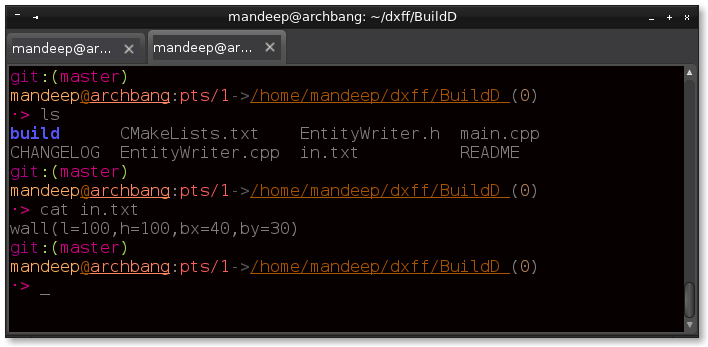
\includegraphics[scale=0.5]{images/bld0.png}
\caption{Input file}
\label{fig:input}
\end{figure}

Then we will compile the project with the help of cmake and make that can be seen in Figure \ref{fig:compile}. It uses the cmake configuration file CMakeLists.txt that's present in the root directory of the project. We have used here the out-of-source build method. That separates the build directory to be separated from the actual source code. For that, a separate directory is created and cmake and make commands are executed there.
After successful build, an executable file will be created with the name BuildD (as specified in the CMakeLists.txt). Hence, we can execute that executable file using ./BuildD.

\begin{figure}
	\centering
	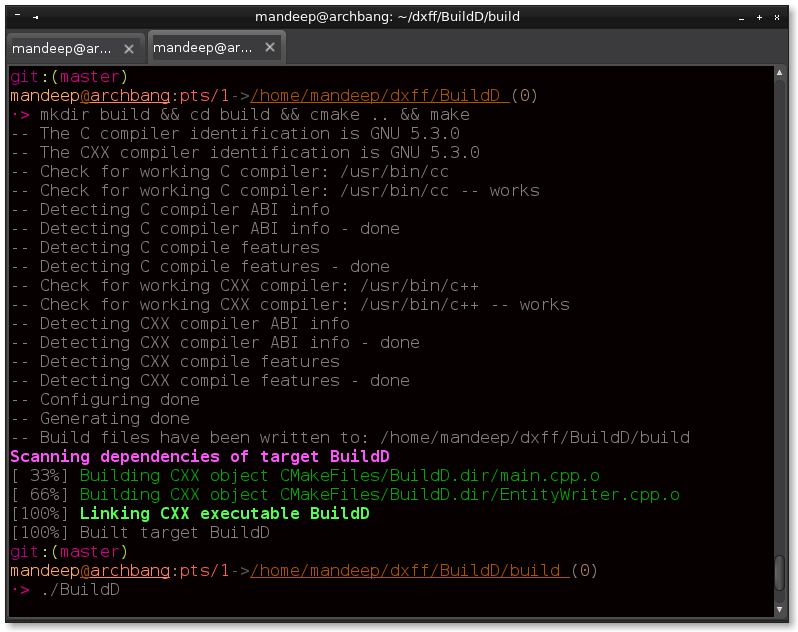
\includegraphics[scale=0.49]{images/bld3.png}
	\caption{Command-line compilation}
	\label{fig:compile}
\end{figure}

Now let's look inside the project and think what's going on actually in there. First the in.txt file is parsed using regular expressions (using Qt libraries) and splitted and joined and stored as an semi-processed output in out.txt file as seen in the Figure \ref{fig:token}. Basically input is divided into smaller tokens and stored in out.txt.

\begin{figure}
\centering
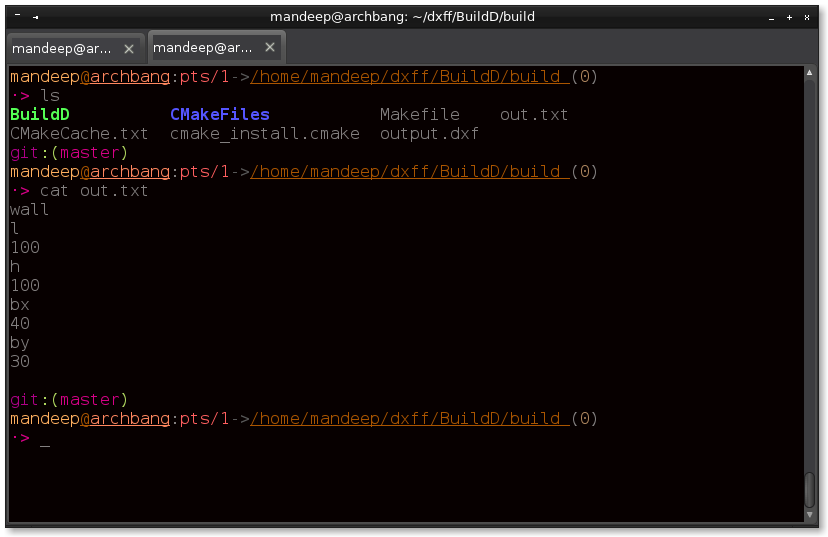
\includegraphics[scale=0.5]{images/bld1.png}
\caption{Tokenized intermediate file}
\label{fig:token}
\end{figure}

We can also work in Qt Creator. It is an IDE for C++ application development that's truly an helping aid with its nice and helping features. You can see the user interface of the Qt Creator in Figure \ref{fig:qt}. It contains a green play button at bottom-left side. One can click that button to build the project and execute the executable file with a single move.

\begin{figure}
\centering
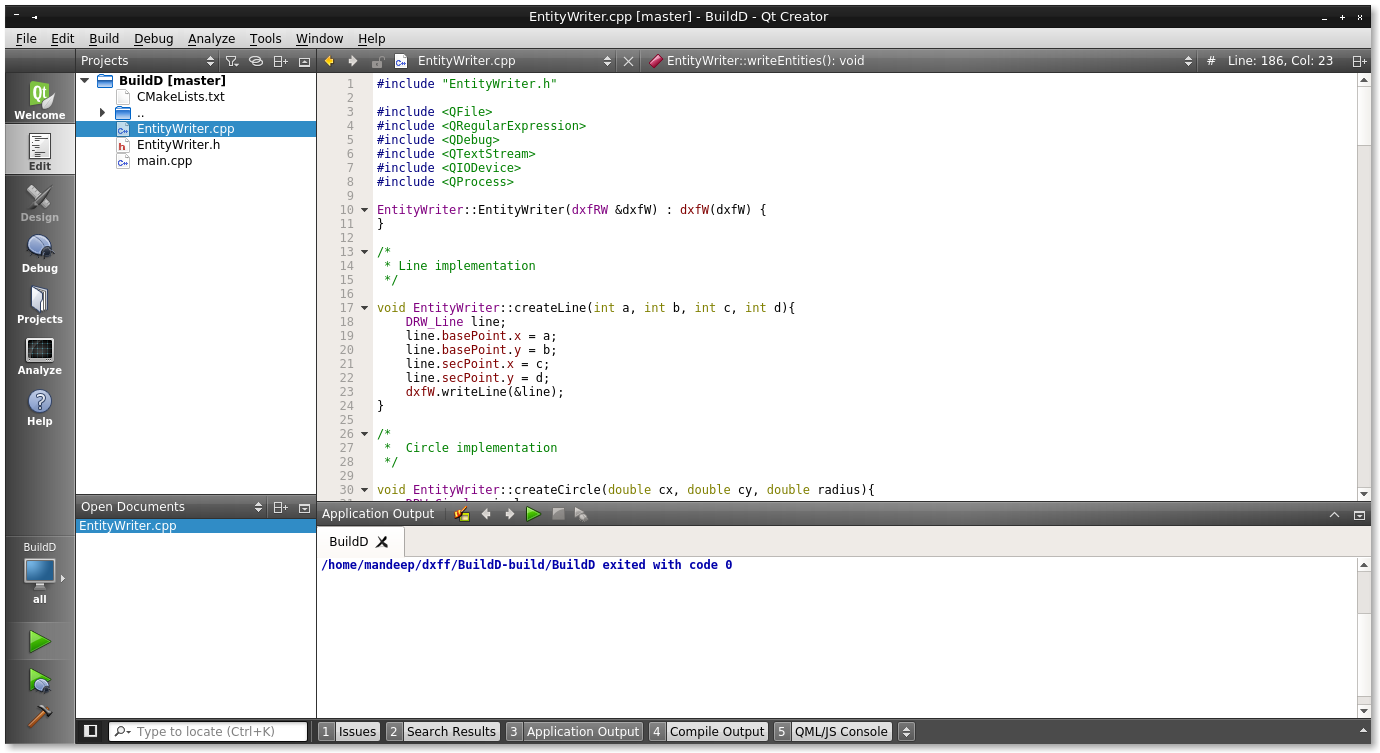
\includegraphics[scale=0.38]{images/bld2.png}
\caption{Qt interface}
\label{fig:qt}
\end{figure}

At the end, we have the final output that will be looking for: the DXF file. It's stored there in the build directory as seen in the Figure \ref{fig:dxf}. It's named as output.dxf. We can open that file in LibreCAD directly from the command-line.


\begin{figure}
\centering
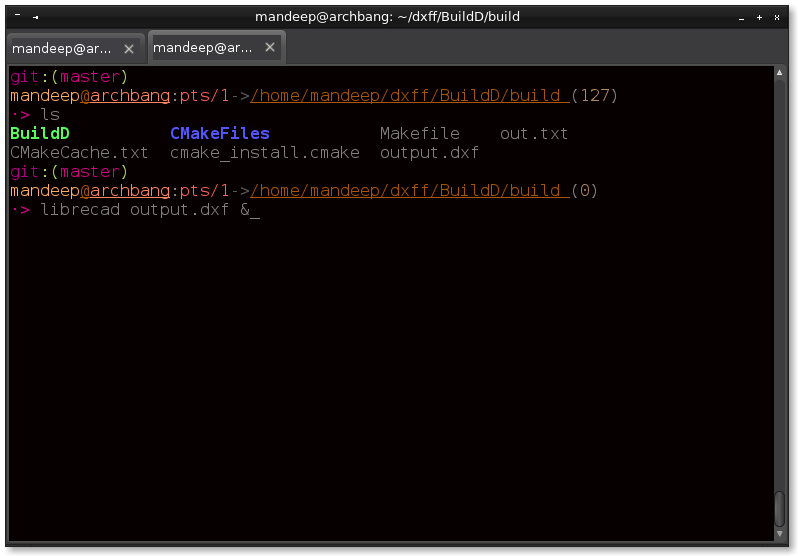
\includegraphics[scale=0.5]{images/bld4.png}
\caption{Opening DXF in LibreCAD from command-line}
\label{fig:dxf}
\end{figure}

Now that our DXF file output.dxf is created and we have issued a command from command-line to open that file in LibreCAD. It can be seen in LibreCAD as shown in Figure \ref{fig:lc}. Although one might need to click the "Auto zoom" feature in LibreCAD to directly view the contents fit to the screen window.

\begin{figure}
\centering
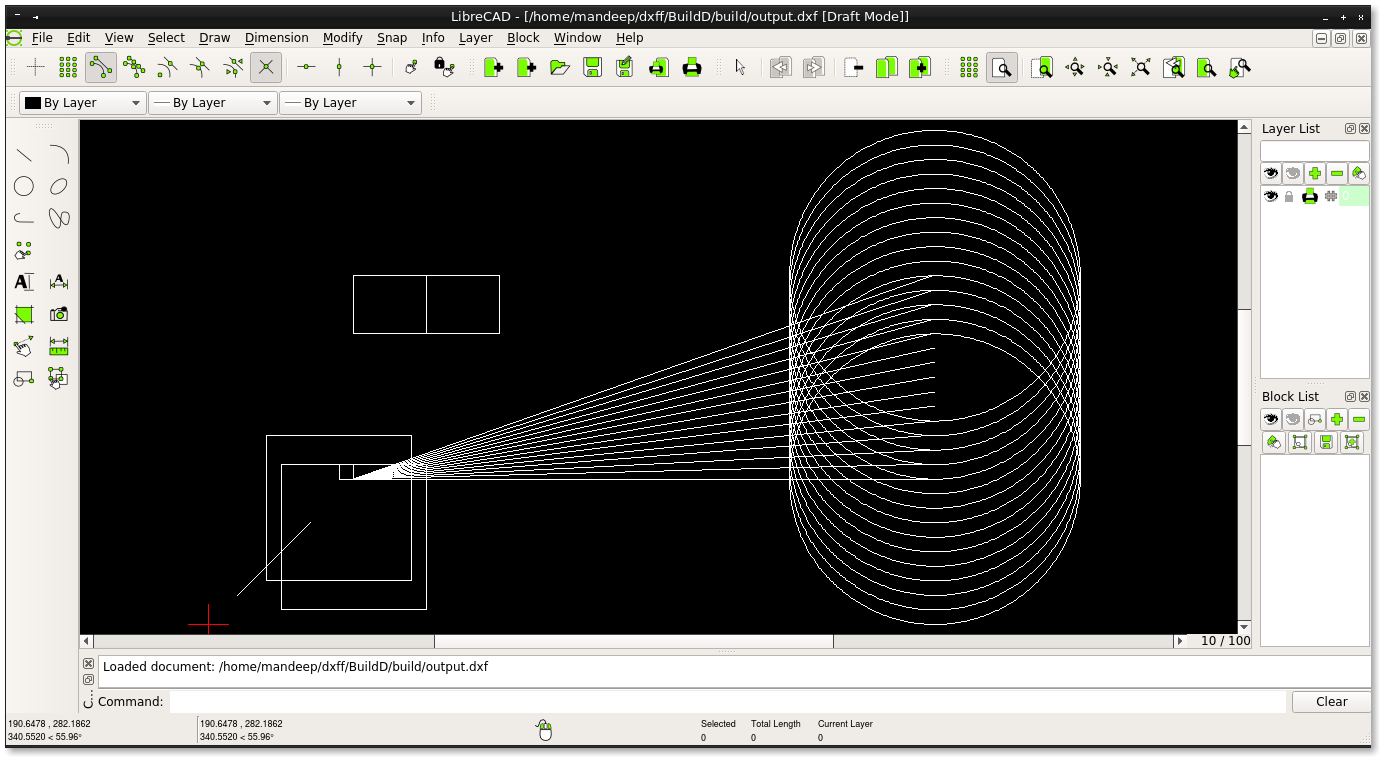
\includegraphics[scale=0.38]{images/bld5.png}
\caption{DXF opened in LibreCAD}
\label{fig:lc}
\end{figure}